% **************************************************************************************************************
% A Classic Thesis Style
% An Homage to The Elements of Typographic Style
%
% Copyright (C) 2015 André Miede http://www.miede.de
%
% If you like the style then I would appreciate a postcard. My address
% can be found in the file ClassicThesis.pdf. A collection of the
% postcards I received so far is available online at
% http://postcards.miede.de
%
% License:
% This program is free software; you can redistribute it and/or modify
% it under the terms of the GNU General Public License as published by
% the Free Software Foundation; either version 2 of the License, or
% (at your option) any later version.
%
% This program is distributed in the hope that it will be useful,
% but WITHOUT ANY WARRANTY; without even the implied warranty of
% MERCHANTABILITY or FITNESS FOR A PARTICULAR PURPOSE.  See the
% GNU General Public License for more details.
%
% You should have received a copy of the GNU General Public License
% along with this program; see the file COPYING.  If not, write to
% the Free Software Foundation, Inc., 59 Temple Place - Suite 330,
% Boston, MA 02111-1307, USA.
%
% **************************************************************************************************************
\RequirePackage{fix-cm} % fix some latex issues see: http://texdoc.net/texmf-dist/doc/latex/base/fixltx2e.pdf
\documentclass[ twoside,openright,titlepage,numbers=noenddot,headinclude,%1headlines,% letterpaper a4paper
                footinclude=true,cleardoublepage=empty,abstractoff, % <--- obsolete, remove (todo)
                BCOR=5mm,paper=a4,fontsize=11pt,%11pt,a4paper,%
                american,spanish%
                ]{scrreprt}

%********************************************************************
% Note: Make all your adjustments in here
%*******************************************************
\input{classicthesis-config}

% # Paquetes
\usepackage{amsthm} % para usar \newtheorem y \proof
\usepackage{mathtools} % para usar rcases
\usepackage{enumitem} % pasa usar tag distintos en las enumeraciones
\usepackage{amssymb} % para usar el simbolo de no divide
\usepackage{xeboiboites} % TODO: añadir ref

% # Definición de estilos de "teoremas":
% # \newtheorem{identificador}{texto}[contador]
% \theoremstyle{plain} % titulo negrita, cuerpo cursiva
\theoremstyle{definition} % titulo negrita, cuerpo en recta
% TODO: ver que hacer
\newtheorem{contador}{contador}[chapter]
% \newtheorem{proposicion}[teorema]{Proposicion}
% \newtheorem{lema}[teorema]{Lema}
% \newtheorem{ejemplo}[teorema]{Ejemplo}
% \newtheorem{definicion}[teorema]{Definición}
% \newtheorem{nota}[teorema]{Nota}
% \newtheorem{ley de grupo}[teorema]{Ley de grupo}
% \newtheorem{algoritmo}[teorema]{Algoritmo}
% \newtheorem{corolario}[teorema]{Corolario}
\newcommand{\nuevoteorema}[3] {
    \newbreakabletheorem[small box style={draw=orange!30!black!20,%
    fill=orange!10!black!2,decoration=penciline, decorate, thick},
    big box style={color=orange!30!black!20,fill=orange!30!black!10,thick},
    broken edges={draw=orange!30!black!20,thick,fill=orange!20!black!5,
    decoration={penciline,segment length=.5cm,%
    amplitude=1.3mm},decorate},%
    other edges={decorate,thick}]%
    {#1}{#2}{#3}
}
\nuevoteorema{teorema}{Teorema}{contador}
\nuevoteorema{proposicion}{Proposición}{contador}
\nuevoteorema{lema}{Lema}{contador}
\nuevoteorema{corolario}{Corolario}{contador}
\nuevoteorema{ley de grupo}{Ley de grupo}{contador}
\nuevoteorema{definicion}{Definición}{contador}
\nuevoteorema{algoritmo}{Algoritmo}{contador}
\nuevoteorema{formulasadiccion}{Fórmulas de adicción}{contador}
%\nuevoteorema{ejemplo}{Ejemplo}{contador}
%\nuevoteorema{nota}{Nota}{contador}
\newtheorem{nota}[contador]{Nota}
\newtheorem{ejemplo}[contador]{Ejemplo}
%\newtheorem{nota}[contador]{Nota}

\nuevoteorema{teorema2}{Teorema}{}


% # Comandos definidos
\newcommand{\F}{\mathbb{F}}
\newcommand{\Fq}{\mathbb{F}_q}
\newcommand{\Fqca}{\overline{\Fq}}
\newcommand{\Fm}{\mathbb{F}_{2^m}}
\newcommand{\Fp}{\mathbb{F}_p}
\renewcommand{\P}{\mathbb{P}}
\newcommand{\A}{\mathbb{A}}
\newcommand{\Kca}{\overline{K}}
\newcommand{\EK}{E(K)}
\newcommand{\EKca}{E(\Kca)}
\newcommand{\EFqca}{E(\Fqca)}
%\newcommand{\deg}{\textrm{deg}}
\newcommand{\dega}{\deg(\alpha)}
%\let\char\relax
\DeclareMathOperator{\car}{char}
\newcommand{\phiq}{\phi_q}


%********************************************************************
% Bibliographies
%*******************************************************
\addbibresource{Bibliography.bib}
%\addbibresource[label=ownpubs]{AMiede_Publications.bib}

%********************************************************************
% Hyphenation
%*******************************************************
%\hyphenation{put special hyphenation here}

% ********************************************************************
% GO!GO!GO! MOVE IT!
%*******************************************************
\begin{document}
\frenchspacing
\raggedbottom
\selectlanguage{spanish} % american ngerman
%\renewcommand*{\bibname}{new name}
%\setbibpreamble{}
\pagenumbering{roman}
\pagestyle{plain}
%********************************************************************
% Frontmatter
%*******************************************************
% TODO: descomentar todo menos Publications
%\include{FrontBackmatter/DirtyTitlepage}
%%*******************************************************
% Titlepage
%*******************************************************
\begin{titlepage}
    % if you want the titlepage to be centered, uncomment and fine-tune the line below (KOMA classes environment)
    \begin{addmargin}[-1cm]{-3cm}
    \begin{center}
        \large

        \hfill

        \vfill

        %\includegraphics[width=0.9\textwidth]{gfx/logo_ugr2.png}\\[1.4cm]
        \includegraphics[width=4cm]{gfx/logo_ugr2} %\\ \medskip

        \vfill

        \spacedallcaps{\mySubtitle} \\ \bigskip

        \spacedlowsmallcaps{\myDegree} \\ \bigskip \bigskip

        % \vfill

        \begingroup
            \color{Maroon}\spacedallcaps{\LARGE\myTitle} \\ \bigskip
        \endgroup

        \vfill

        \textbf{Autor} \\
        \myName \\ \medskip

        \textbf{Tutor} \\
        \myProf \\ \medskip

        \vfill

        %\myDepartment \\
        \spacedlowsmallcaps{\myUni} \\ \medskip
        %\spacedlowsmallcaps{\myFaculty} \\
        %\spacedlowsmallcaps{\myOtherFaculty} \\ \bigskip
        %\myUni \\ \bigskip

        \myLocation, \myTime %\ -- \myVersion

        \vfill

    \end{center}
  \end{addmargin}
\end{titlepage}

%%*******************************************************
% Titlepage
%*******************************************************
\begin{titlepage}
    % if you want the titlepage to be centered, uncomment and fine-tune the line below (KOMA classes environment)
    \begin{addmargin}[-1cm]{-3cm}
    \begin{center}
        \large

        \hfill

        \vfill

        % \vfill

        \begingroup
            \color{Maroon}\spacedallcaps{\LARGE\myTitle} \\ \bigskip
        \endgroup

        \vfill

        \textbf{Autor} \\
        \myName \\ \medskip

        \textbf{Director} \\
        \myProf \\ \medskip

    \end{center}
  \end{addmargin}
\end{titlepage}

% \thispagestyle{empty}
%
% \hfill
%
% \vfill
%
% \noindent\myName: \textit{\myTitle,} \mySubtitle, %\myDegree,
% \textcopyright\ \myTime
%
% %\bigskip
% %
% %\noindent\spacedlowsmallcaps{Supervisors}: \\
% %\myProf \\
% %\myOtherProf \\
% %\mySupervisor
% %
% %\medskip
% %
% %\noindent\spacedlowsmallcaps{Location}: \\
% %\myLocation
% %
% %\medskip
% %
% %\noindent\spacedlowsmallcaps{Time Frame}: \\
% %\myTime

%\cleardoublepage\include{FrontBackmatter/Dedication}
%\cleardoublepage\include{FrontBackmatter/Foreword}
%\cleardoublepage%*******************************************************
% Abstract
%*******************************************************
%\renewcommand{\abstractname}{Abstract}
\pdfbookmark[1]{Resumen}{Resumen}
\begingroup
\let\clearpage\relax
\let\cleardoublepage\relax
\let\cleardoublepage\relax

\chapter*{Resumen}
Resumen

\medskip

\textbf{Palabras clave}: ...

\vfill

%\begin{otherlanguage}{american}
%\pdfbookmark[1]{Zusammenfassung}{Zusammenfassung}
\chapter*{Abstract}
Abstract.

\medskip

\textbf{Keywords}: ...

%\end{otherlanguage}

\endgroup

\vfill

%\cleardoublepage\include{FrontBackmatter/Publications}
%\cleardoublepage%*******************************************************
% Acknowledgments
%*******************************************************
\pdfbookmark[1]{Agradecimientos}{agradecimientos}

% \begin{flushright}{\slshape
%     We have seen that computer programming is an art, \\
%     because it applies accumulated knowledge to the world, \\
%     because it requires skill and ingenuity, and especially \\
%     because it produces objects of beauty.} \\ \medskip
%     --- \defcitealias{knuth:1974}{Donald E. Knuth}\citetalias{knuth:1974} \citep{knuth:1974}
% \end{flushright}

\begingroup
\let\clearpage\relax
\let\cleardoublepage\relax
\let\cleardoublepage\relax
\chapter*{Agradecimientos}

Quería agradecer en primer lugar a la Universidad de Granada y sus profesores, por darme la oportunidad de formarme. En especial, al tutor de este trabajo, Pascual Jara, por su ayuda constante a lo largo de este proyecto.

\bigskip

Finalmente, mi mayor agradecimiento a mi familia por no dejar de apoyarme nunca.

\endgroup

\pagestyle{scrheadings}
\cleardoublepage\include{FrontBackmatter/Contents}
%********************************************************************
% Mainmatter
%*******************************************************
\cleardoublepage\pagenumbering{arabic}
%\setcounter{page}{90}
% use \cleardoublepage here to avoid problems with pdfbookmark
\cleardoublepage
%\part{Prefacio}
%%********************************************
\chapter{Ejemplo de cosas que se pueden hacer}\label{ch:introducción}
%********************************************

\marginpar{Ejemplo comentario al margen}

Ejemplo cita 1 \citeauthor{bringhurst:2002} % no sale enlace

Ejemplo cita 2 \citep{bringhurst:2002} % si sale

Ejemplo cita 3 \cite{bringhurst:2002} % si sale

Enlace a pie de pagina \footnote{Pie de página}

\emph{Curiva}, \texttt{maquina}, \textit{itálica}, \spacedallcaps{All Caps},  \textsc{Small Caps}, \spacedlowsmallcaps{Low Small Caps}.

Comentarios de algo de \verb|tex|.

Ejemplo en latín \eg

Acrónimos: \ac{UML}, \acs{UML} ,\acf{UML}, \acp{UML}

\paragraph{Párafro:} Lorem ipsum dolor sit amet, consectetur adipiscing elit. Integer vitae dapibus orci. Cras vel nunc mattis, lobortis sapien sit amet, pharetra enim. Nullam bibendum libero in sodales faucibus. Nullam risus mi, vehicula in metus ut, tristique molestie mauris. Nullam a sem augue. Sed tincidunt rutrum leo at tempor.

\subsection{Subsección}
\graffito{Comentario justo al lado del título de la sección}

\begin{table}[h]
  \myfloatalign
  \begin{tabularx}{\textwidth}{Xl} \toprule
    \tableheadline{head1 expandido} & \tableheadline{head2}  \\
    \midrule
    1 & 2 \\
    3 & 4 \\
    %postulant quo & westeuropee & sanctificatec \\
    \midrule
    5 & 6 \citeauthor{knuth:1976} \\
    \bottomrule
  \end{tabularx}
  \caption[Ejemplo de tabla 1]{Ejemplo de tabla 1}  \label{tab:example}
\end{table}

\begin{tabular}{ll}
$\rho$       & rho \\
$ \delta x$  & delta x \\
Ejemplo de tabla 2 &
\end{tabular}

% enlarga esta página (por abajo 2 cent): \enlargethispage{2cm}

\begin{figure}[h]
  \myfloatalign
  \subfloat[Imagen 1]
  {\includegraphics[width=.45\linewidth]{gfx/example_1}} \quad
  \subfloat[Imagen 2]
  {\includegraphics[width=.45\linewidth]{gfx/example_2}}
  \caption[Ejemplo figure]{Ejemplo figure}\label{fig:example}
\end{figure}

\begin{equation}
  x = 2 \quad (\textrm{texto})
\end{equation}

\begin{eqnarray*}
  x = 3 \\
  y = 4
\end{eqnarray*}

Referencia: \autoref{tab:example} y \autoref{ch:introducción}

\clearpage % new page

\cleardoublepage
%\ctparttext{Desarollo del trabajo matemático-informático.}
%\part{Desarollo del trabajo}
%**************************
\chapter{Aritmética de las curvas elíptica}
\label{ch:Aritmética de las curvas elíptica}
%**************************

% conceptos han aparecido: extensión de cuerpo, característica

En el apartado~\ref{sec:Introducción} se introducen las curvas elípticas. Se explican las operaciones de grupo adicción y duplicacíon para los puntos de una curva elíptica, junto con su estructura fundamental y otras propiedades.

Las principales referencias usadas en este capítulo han sido~\cite{Washington:2008} y~\cite{Hankerson:2003}.

% TODO: seguir con la introducción de contenidos

\section{Introducción a las curvas elípticas}
\label{sec:Introducción}

% TODO: preguntarle a Pascual por la forma de citar (poner en el encabezado las principales referencias y despues para cosas puntuales usar \cite), pero no en cada definición o resultado no trivial.
\begin{definicion}
\label{def:curva elíptica}
	Una \emph{curva elíptica} $E$ se define por una una ecuación de la forma
	\begin{equation}
	\label{eq:Weierstrass general}
		E : y^2 + a_1 x y + a_3 y = x^3 + a_2 x^2 + a_4 x + a_6
	\end{equation}

	donde $a_1, a_2, a_3, a_4, a_6 \in K$ y $\Delta \neq 0$, donde $\Delta$ es el \emph{discriminante} de $E$ y se define como:

	\begin{align}
		\label{eq:discriminante}
		\begin{rcases}
		\Delta & = -d_2^2 d_8 - 8 d_4^3 - 27 d_6^2 + 9 d_2 d_4 d_6         \\
		d_2    & = a_1^2 + 4 a_ 2                                          \\
		d_4    & = 2 a_4 + 4 a_2                                           \\
		d_6    & = a_3^2 + 4 a_6                                           \\
		d_8    & = a_1^2 a_6 + 4 a_2 a_6 - a_1 a_3 a_4 + a_2 a_3^2 - a_4^2 \\
		\end{rcases}
	\end{align}

	Si $L$ es una extensión del cuerpo $K$, entonces el conjunto de puntos \emph{L-racionales} de $E$ es:
	$$
	E(L) = \{\infty\} \cup \{(x, y) \in L \times L: y^2 + a_1 x y + a_3 y = x^3 + a_2 x^2 + a_4 x + a_6 = 0\}
	$$
\end{definicion}

\begin{nota}[comentarios de la definición~\ref{def:curva elíptica}]\leavevmode
	\begin{itemize}
		\item La ecuación~\eqref{eq:Weierstrass general} se conoce como la \emph{ecuación de Weierstrass}.
		\item Diremos que $E$ \emph{está definida sobre} $K$ y lo notaremos $E/K$. A $K$ lo llamaremos \emph{cuerpo base}.
		\item La condición $\Delta \neq 0$ asegura que la curva elíptica es <<suave>>, esto es, no hay puntos en los que la curva tenga dos o mas rectas tangentes.
		% TODO: rellenar referencia a la forma proyectiva
		% TODO: cambiar si no se hace referencia al proyectivo (página 25 de washington)
		\item El punto $\infty$ es el único punto en la línea del infinito que satisface la forma proyectiva de la ecuación de Weierstrass (véase~\ref{}).
	\end{itemize}
\end{nota}

\begin{ejemplo}[curvas elípticas sobre $\mathbb{R}$]
	Consideramos las curvas elípticas:
	\begin{align*}
		E_1: y^2 & = x^3 - x \\
		E_2: y^2 & = x^3 + x
	\end{align*}
	definidas sobre el cuerpo $\mathbb{R}$ de los números reales. Los puntos $E_1(\mathbb{R})$ y $E_2(\mathbb{R})$ se han representado en la Figura~\ref{fig:curvas elípticas reales}.

	% TODO:hacer la gráfica bien (añadir label, etc, etc)
	\begin{figure}[h]
		\myfloatalign
		\subfloat[$E_1: y^2 = x^3 - x$]
		{\includegraphics[width=.45\linewidth]{gfx/grafo_curva_eliptica_reales_1.pdf}} \quad
		\subfloat[$E_2: y^2 = x^3 + x$]
		{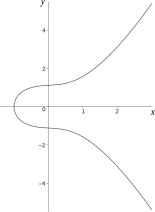
\includegraphics[width=.45\linewidth]{gfx/grafo_curva_eliptica_reales_2.pdf}}
		\caption{Curvas elípticas sobre $\mathbb{R}$}\label{fig:curvas elípticas reales}
	\end{figure}

	% \begin{figure}[h]
	% 	\centering
	% 	\includegraphics[scale=1]{gfx/example_1}
	% 	\caption{Curvas elípticas sobre $\mathbb{R}$}\label{fig:curvas elípticas reales}
	% \end{figure}
\end{ejemplo}

\subsection{Ecuaciones de Weierstrass simplificadas}
\label{sub:Ecuaciones de Weierstrass simplificadas}

\begin{definicion}
	Dos curvas elípticas $E_1$ y $E_2$ definidas sobre $K$ y dadas por las ecuaciones de Weierstrass:
	\begin{align*}
		E_1 &: y^2 + a_1 x y + a_3 y = x^3 + a_2 x^2 + a_4 x + a_6 \\
		E_2 &: y^2 + a_1' x y + a_3' y = x^3 + a_2' x^2 + a_4' x + a_6'
	\end{align*}
	se dicen que son \emph{isomorfas sobre K} si existen $u, r, s, t \in K,\ u \neq 0$, tal que el cambio de variables lineal
	\begin{equation}\label{eq:cambio de variables admisible}
	(x, y) \mapsto (u^2 x + r, u^3 y + u^2 s x + y)
	\end{equation}
	transforma la ecuación $E_1$ en la ecuación $E_2$. La transformación~\eqref{eq:cambio de variables admisible} se llama un cambio de variables admisible.

	El cambio de variables~\eqref{eq:cambio de variables admisible} es el único que deja <<fijo>> el punto del infinito y preserva la forma de la ecuación de Weierstrass. No vamos a entrar en más detalle, pero puede consultar \cite[prop. III.3.1b]{Silverman:2009} para más informácion.
\end{definicion}

% TODO: explicar porqué este cambio de variable referenciando a silverman

Una ecuación de Weierstrass
$$
E:  y^2 + a_1 x y + a_3 y = x^3 + a_2 x^2 + a_4 x + a_6
$$
puede simplificarse considerablemente aplicando cambios de variables admisibles. Usaremos las ecuaciones simplificadas en vez de la general en el resto del trabajo. Vamos a considerar por separado los casos en los que el cuerpo base tenga característica distinta de 2 y 3 o tenga característica 2 o 3.

\begin{enumerate}
	\item Si la característica de $K$ es distinta de $2$ y $3$, entonces el cambio de variables admisible
	$$
	(x, y) \mapsto \left(\frac{x - 3 a_1^2 - 12 a_2}{36}, \frac{y - 3 a_1 x}{216} - \frac{a_1^3 + 4 a_1 a_2 - 12 a_3}{240}\right)
	$$
	transforma $E$ en la curva
	\begin{equation*}\label{eq:ecuación Weierstrass}
		y^2 = x^3 + a x + b
	\end{equation*}
	donde $a, b \in K$. El discriminante de esta curva es $\Delta = -16(4a^3 + 27b^2)$.

	\item Si la característica de K es 2, hay dos casos que considerar. Si $a_1 \neq 0$, entonces el cambio de variables admisible
	$$
	(x, y) \mapsto \left(a_1^2 x + \frac{a_3}{a_1}, a_1^3 y + \frac{a_1^2 a_4 + a_3^2}{a_1^3} \right)
	$$
	transforma $E$ en la curva
	\begin{equation*}
		y^2 + xy = x^3 + a x^2 + b
	\end{equation*}
	% TODO: rellenar referencia
	donde $a, b \in K$. Tales curvas se llaman \emph{no supersingulares} (véase~\ref{}) y tiene discriminante $\Delta = b$. Si $a_1 = 0$, entonces el cambio de variables admisible
	$$
	(x, y) \mapsto (x + a_2, y)
	$$
	transforma $E$ en la curva
	\begin{equation*}
		y^2 + c y = x^3 + a x + b
	\end{equation*}
	% TODO: rellenar referencia
	donde $a, b, c \in K$. Tales curvas se llaman \emph{supersingulares} (véase~\ref{}) y tiene discriminante $\Delta = c^4$.

	\item Si la característica de $K$ es 4, entonces hay dos casos que considerar. Si $a_1^2 \neq -a_2$, entonces el cambio de variables admisible
	$$
	(x, y) \mapsto \left(x + \frac{d_4}{d_2}, y + a_1 x + a_1 \frac{d_4}{d_2} + a_3 \right)
	$$
	donde $d_2 = a_1^2 + a_2$ y $d_4 = a_4 - a_1 a_3$, transforma $E$ en la curva
	\begin{equation*}
		y^2 = x^3 + a x^2 + b
	\end{equation*}
	% TODO: rellenar referencia
	donde $a, b \in K$. Tales curvas se llaman \emph{no supersingulares} (véase~\ref{}) y tiene discriminante $\Delta = -a^3 b$. Si $a_1^2 = -a_2$, entonces el cambio de variables admisible
	$$
	(x, y) \mapsto (x, y + a_1 x + a_3)
	$$
	transforma $E$ en la curva
	\begin{equation*}
		y^2 = x^3 + a x^2 + b
	\end{equation*}
	% TODO: rellenar referencia
	donde $a, b \in K$. Tales curvas se llaman \emph{supersingulares} (véase~\ref{}) y tiene discriminante $\Delta = -a^3$.
\end{enumerate}
\begin{proof}
La demostración completa puede encontrarse en~\cite[sec. III.1]{Silverman:2009}. Se trata simplemente de completar cuadrados y realizar sustituciones, por ello aquí solo mostraremos la demostración de la primera simplifación.

En primer lugar, sumando en la ecuación de Weierstrass~\eqref{eq:Weierstrass general} en ambos lados por $(a_1 a_3 x)/2 + a_3^2/4 + (a_1^2 x^2)/4$, completamos el cuadrado:
$$
\left(y + \frac{a_1 x}{2} + \frac{a_3}{2}\right)^2 = x^3 + \left(a_2 + \frac{a_1^2}{4}\right)x^2 + \left(a_4 + \frac{a_1 a_3}{2}\right)x + \left(a_6 + \frac{a_3^2}{4}\right)
$$
Haciendo $y_1 = y + \frac{a_1 x}{2} + \frac{a_3}{2}$, obtenemos
$$
y_1^2 = x^3 + a_2' x^2 + a_4' x + a_6'
$$
para algunas constantes $a_2', a_4', a_6' \in K$. Finalmente, sustituyendo $x_1 = x + \frac{a_2'}{3}$ resulta
$$
y_1^2 = x_1^3 + a x_1 + b
$$
para algunas constante $a, b \in K$. Para obtener el discriminante $\Delta$ basta sustiuir el valor de las constantes $a_4 = a,\ a_6 = b$ y $a_1 = a_3 = a_2 = 0$ en~\eqref{eq:discriminante}.
\end{proof}

\subsection{Ley de grupo}
\label{sub:Ley de grupo}

Sea $E$ una curva elíptica definida sobre un cuerpo $K$. Hay un \emph{método de la cuerda y la tangente} para sumar dos puntos en $E(K)$ y obtener un tercer punto en $E(K)$. Junto con esta operación aditiva, el conjunto de puntos $E(K)$ forma un gurpo abeliano con $\infty$ como elemento neutro.

La regla aditiva se explica fácilmente geométricamente. Sea $P$ y $Q$ dos puntos distintos de una curva elíptica $E$. Entonces la \emph{suma} $R$, de $P$ y $Q$ esta definido como sigue. Se dibuja una recta $L$ de $P$ a $Q$. Esta recta intersecta la curva elíptica en un tercer punto. Entonces $R$ es la reflexión de este punto sobre el eje-$x$. Esto se puede apreciar en la Figura~\ref{fig:ejemplo adicción}.

El \emph{doble} $R$, de $P$, se define como sigue. Se dibuja la línea tangente $L$ a la curva elíptica en $P$. Esta línea intersecta la curva elíptica en un segundo punto. Entonces $R$ es la reflexión de esto punto sobre el eje-$x$. Esto se puede apreciar en la Figura~\ref{fig:ejemplo duplicación}.

\begin{figure}[h]
  \myfloatalign
  \subfloat[Adicción: $P + Q = R$]{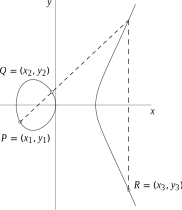
\includegraphics[width=.45\linewidth]{gfx/ejemplo_adiccion.pdf}\label{fig:ejemplo adicción}}
  \quad
  \subfloat[Duplicación: $P + P = P$]{\includegraphics[width=.45\linewidth]{gfx/ejemplo_duplicacion.pdf}\label{fig:ejemplo duplicación}}
  \caption{Adicción y duplicación geométrica de puntos de una curva elíptica}\label{fig:Adicción y duplicación geométrica de puntos de una curva elíptica}
\end{figure}

El hecho de que $L \cap E$, contando multiplicidades, consiste en exactamente tres puntos (no necesariamente distintos) es un caso especial del teorema de Bézout~\cite[sec. I.7.8]{Hartshorne:1977}. Sin embargo, como vamos a dar fórmulas explícitas posteriormente en esta sección, no hay necesidad de usar un teorema general.

%\include{Chapters/Chapter02}
%\addtocontents{toc}{\protect\clearpage} % <--- just debug stuff, ignore
%\include{Chapters/Chapter03}
%\include{multiToC} % <--- just debug stuff, ignore for your documents
% ********************************************************************
% Backmatter
%*******************************************************
\appendix
%\renewcommand{\thechapter}{\alph{chapter}}
%\cleardoublepage
%\part{Apéndice}
%\include{Chapters/Chapter0A}
%********************************************************************
% Other Stuff in the Back
%*******************************************************
%cleardoublepage\include{FrontBackmatter/Bibliography}
%\cleardoublepage\include{FrontBackmatter/Declaration}
%\cleardoublepage\include{FrontBackmatter/Colophon}
% ********************************************************************
% Game Over: Restore, Restart, or Quit?
%*******************************************************
\end{document}
% ********************************************************************
